\documentclass[12pt]{article}

\newcommand{\name}{Mike Gao}
\newcommand{\problemset}{ MIDTERM }

%\pagestyle{headings}
\usepackage[dvips]{graphics,color}
\usepackage{amsfonts}
\usepackage{amssymb}
\usepackage{amsmath}
\usepackage{latexsym}
\usepackage{enumerate}
\usepackage{graphicx}
\setlength{\parskip}{1pc}
\setlength{\parindent}{0pt}
\setlength{\topmargin}{-3pc}
\setlength{\textheight}{9.5in}
\setlength{\oddsidemargin}{0pc}
\setlength{\evensidemargin}{0pc}
\setlength{\textwidth}{6.5in}
\usepackage{minted}
\newcommand{\answer}[1]{
\newpage
\noindent
\framebox{
	\vbox{
		COMP 557 \hfill {\bf \problemset} \hfill Prof. Paul Kry \\ 
		\name \hfill \today \\
		260915701 \hfill \# #1
	}
}
\bigskip

}
\usepackage{xcolor}

\usemintedstyle{friendly}

\begin{document}


% PROBLEM 1

\answer{1 -- Coordinate Frame}

\begin{minted}{glsl}
// normal vector is n, n dot p is the point, let s, t be coordinates
Matrix4d coordFrame( const Vec3f &n, const Vec3f &p)
{
  Vec3f s,t;
  // if n is near x axis
  if(n.x > 0.9f) {
    s = Vec3f (0.0 f, 1.0 f, 0.0 f );
  } else {
    s = Vec3f (1.0 f, 0.0 f, 0.0 f);
  }
  s -= n* dot(s, n); // make s orthogonal to n
  s *= rsqrt(dot(s, s)); // normalize s
  t = cross(n, s);
  return (new double[] {
    t.x, s.x, n.x, p.x,
    t.y, s.y, n.y, p.y,
    t.z, s.z, n.z, p.z
    0, 0, 0, 1
  })
}
\end{minted}


% PROBLEM 2

\answer{2 --  Rotation Using Similarity Transform}


Assume the axis pass through two points, $P_1=(x_1, y_1, z_1)$ and $P_2=(x_2,y_2,z_2)$
\begin{enumerate}[(1)]

\item
Create the axis passing through origin by translating space by $-P_1$ for example

$ T = \begin{pmatrix}
1 & 0 & 0 & -x_1\\
0 & 1 & 0 & -y_1\\
0 & 0 & 1 & -z_1\\
0 & 0 & 0 & 1
\end{pmatrix}$

\item
Rotate space about the x axis so that the rotation axis lies in the xz plane.

Let u be a unit vector $(p,q,r)$ along the rotation axis. 

Project $u$ onto yz-plane, let $s=\sqrt{q^2+r^2}$ be the length of the projection. Rotate by $\alpha$ in order to get $u$ in xz-plane

$cos\alpha = \frac{r}{s} $ $sin\alpha = \frac{q}{s}$
$ Rx = \begin{pmatrix}
1 & 0 & 0 & 0\\
0 & \frac{r}{s} & -\frac{q}{s} & 0\\
0 & \frac{q}{s} & \frac{r}{s} & 0\\
0 & 0 & 0 & 1
\end{pmatrix}$

\item
We then rotate by $\beta$ so the axis overlap the z-axis:

$cos\beta = \frac{s}{||u||}= s$ $sin\beta = \frac{-p}{||u||} = -p $

$ Ry = \begin{pmatrix}
s & 0 & -p & 0\\
0 & 1 & 0 & 0\\
p & 0 & s & 0\\
0 & 0 & 0 & 1
\end{pmatrix}$

\item
We then rotate around z-axis by the given angle $\theta$

$ Rz = \begin{pmatrix}
cos\theta & -sin\theta & 0 & 0\\
sin\theta & cos\theta & 0 & 0\\
0 & 0 & 1 & 0\\
0 & 0 & 0 & 1
\end{pmatrix}$

Finally, $p'=T^{-1}R_x^{-1}R_y^{-1}R_zR_yR_xTp$
\end{enumerate}



% PROBLEM 3

\answer{3 -- Perspective Projection Matrix}

$ P = \begin{pmatrix}
n & 0 & 0 & 0\\
0 & n & 0 & 0\\
0 & 0 & n & 0\\
0 & 0 & -1 & 0
\end{pmatrix}$

Where this will take in point $(x, y, z, 1)^T$ to $(nx, ny, nz, -z)^T$, After dividing by the $z$ coordinate we have $(-nx/z,-ny/z,-n,1)$ which is the desired point of the near plane



% PROBLEM 4

\answer{4 -- Creating Similarity Transform to Provide Cheap Shadow Projection}

\begin{center}
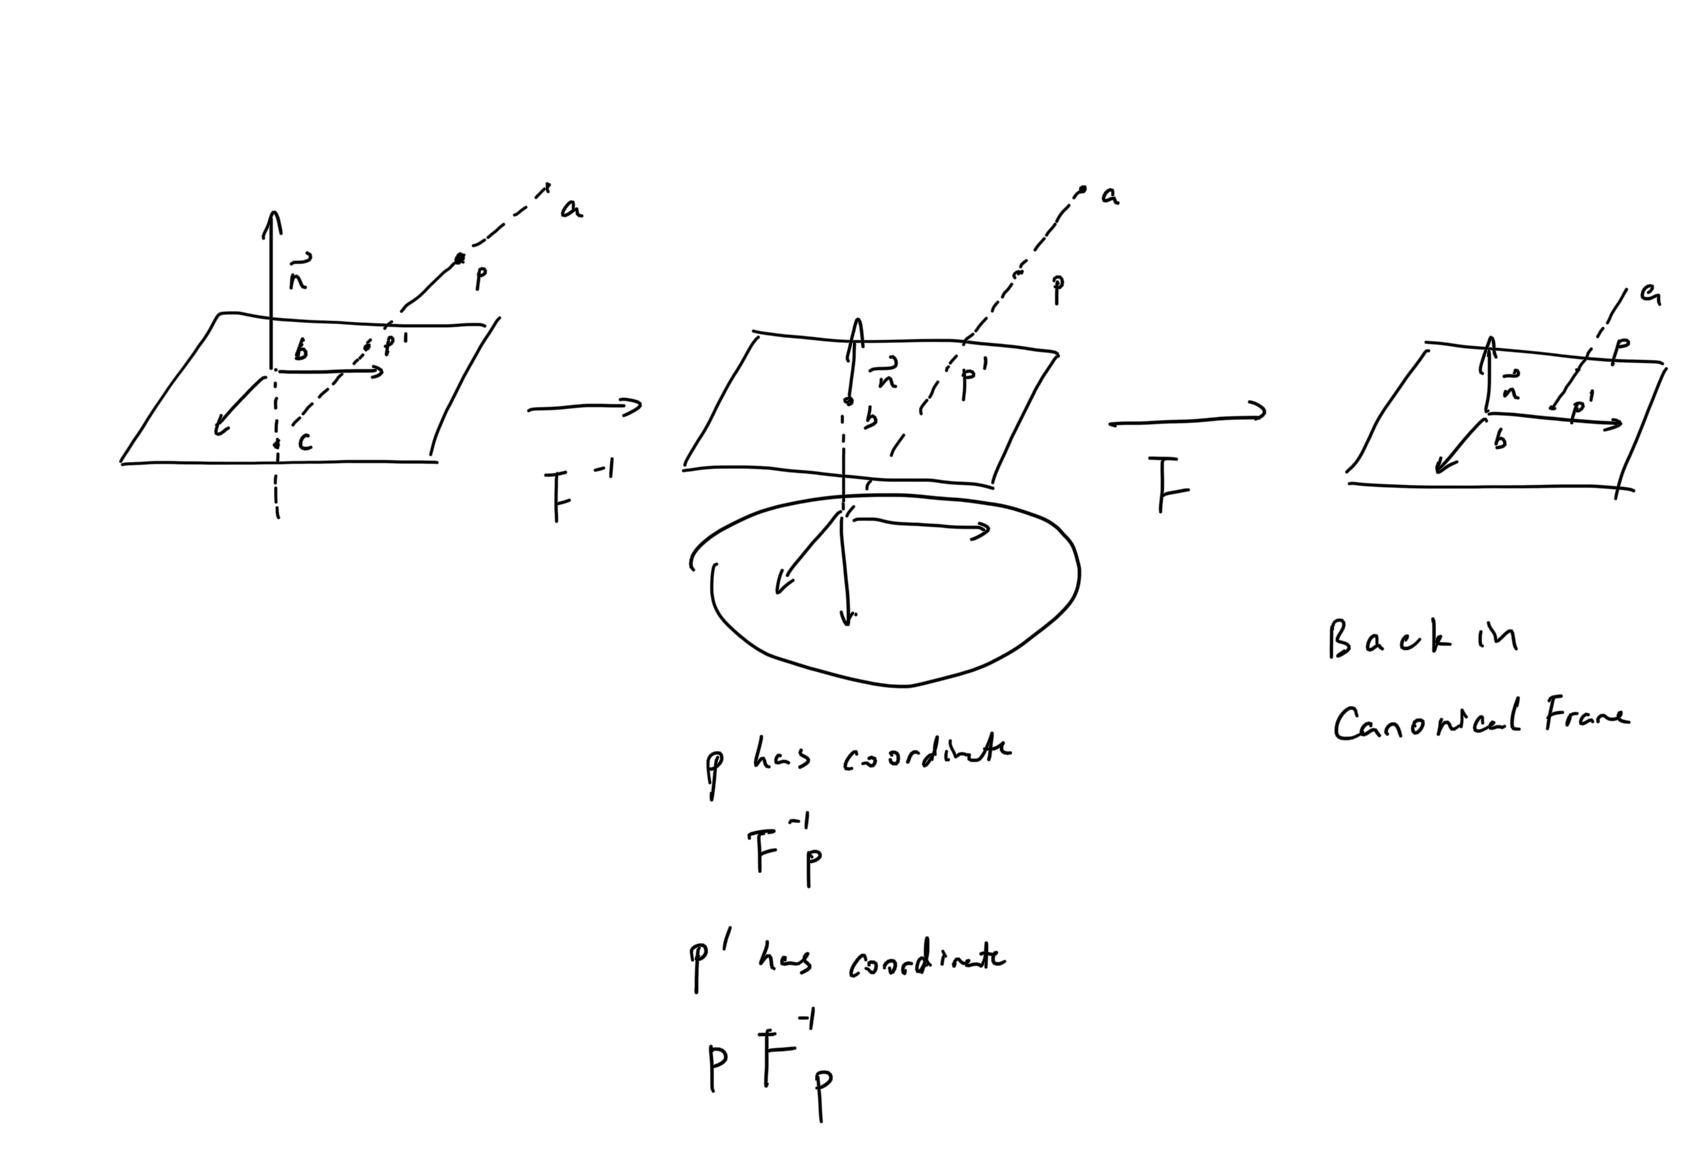
\includegraphics[width=13cm, height=10cm]{q4-diagram.png}
\end{center}

As shown in (1) a point light project point $p\in \mathbb{R}^3$ onto the plane with normal $n$ at $p'$. We let x be the origin of the canonical basis and $n$ be the z-axis

$L_{LP} = L + (p-L)t$

$L_n = x+nt$

We let $L_{LP} = L_n$ and find their intersection point $o$.

Case 1:
If $o$ above $x$, then by Q1 we can construct a new frame, and its frame matrix $F$ by point o and $\vec{n}$ then consider the plane to be the near plane with distance n. 

The coordinate of p is $F^{-1}p$, and projection $PF^{-1}p$, where P is the projection matrix from Q3. Using similarity transform, $p'=FPF^{-1}p$ in the canonical basis

Case 2:
If $o$ is below $x$ then construct $F$ with $o$ and $-\vec{n}$, we can get $p' = FPF^{-1}p$

Case 3:
If $o$ is at x, then $p' = x$

% PROBLEM 5

\answer{5 -- What is the closest near plane you can set?}

Let $s=\begin{pmatrix}0\\0\\-1\\1\end{pmatrix}$ be a point on the quadrilateral, and $t=\begin{pmatrix}0\\0\\-2\\1\end{pmatrix}$ be a point on the wall.

$P =\begin{pmatrix}n&0&0&0\\0&n&0&0\\0&0&n+10&10n\\0&0&-1&0\end{pmatrix}$

$P_s = \begin{pmatrix}0\\0\\-n-10+10n\\1\end{pmatrix}$

$P_t = \begin{pmatrix}0\\0\\-2n-20+10n\\2\end{pmatrix} =  \begin{pmatrix}0\\0\\-n-10+5n\\1\end{pmatrix}$

We are only concerned about the z coordinates of those points

$z_{P_s} = -n-10+10n$

$z_{P_t} = -n-10+5n$

We want to minimize, i.e $|z_{P_s} - z_{P_t}| = \epsilon$ so:

$|-n-10+10n-(-n-10+5n)| = \epsilon$

$|5n| = \epsilon$

$n=\frac{\epsilon}{5}$

% PROBLEM 6

\answer{6 -- Where Should the Point Light Be Placed?}
\begin{center}
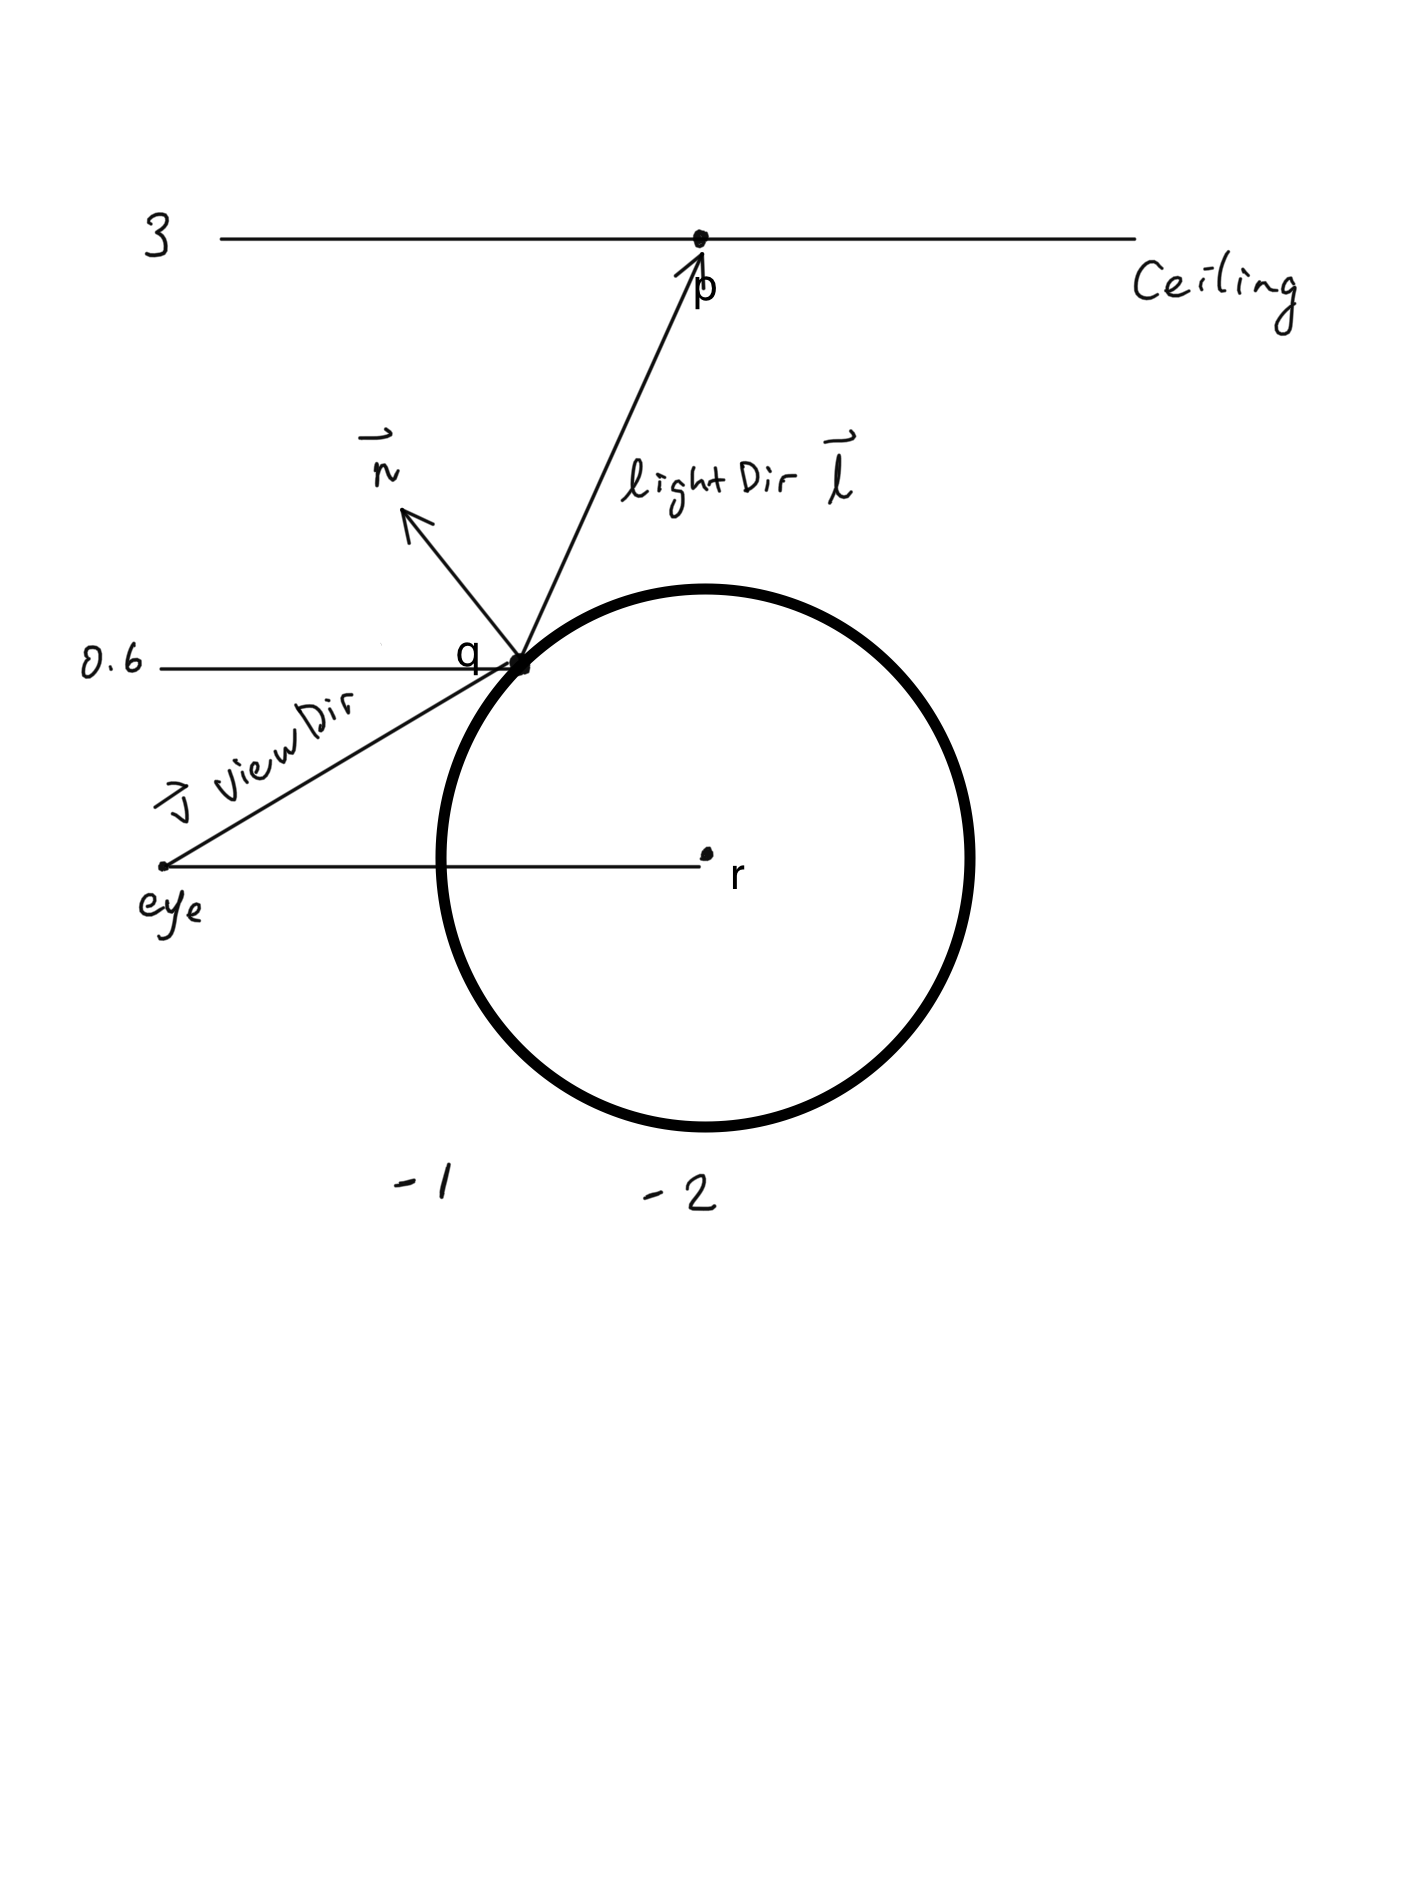
\includegraphics[width=14cm, height=19cm]{q6-diagram.png}
\end{center}
Where p is the light position (unknown), r is the center of the circle, q is the brightest spot of a
Blinn-Phong specular highlight.

We need to find the position of $q$ first. Since we know $y_q = 0.6$, we get:

$x_q^2+0.6^2=1$

$x_q =0.8$

Thus, $z_q = -2+0.8 = 1.2$

Now we can find the view direction $v$ and the normal $n$.

$n = q-r = \begin{pmatrix}0 \\0.6\\0.8\\0\end{pmatrix}$

$v = eye - q = \begin{pmatrix}0 \\-0.6\\1.2\\0\end{pmatrix}$

Now let's find $l$. Suppose $u$ is a vector such that $v - 2u = l$

$u = v - proj_n v = \begin{pmatrix}0 \\-0.6\\1.2\\0\end{pmatrix}- \begin{pmatrix}0\\0.36\\0.48\\0\end{pmatrix} =\begin{pmatrix}0\\-0.96\\0.72\\0\end{pmatrix}$


$l = v-2u=\begin{pmatrix}0 \\-0.6\\1.2\\0\end{pmatrix}-2\begin{pmatrix}0 \\-0.96\\0.72\\0\end{pmatrix}=\begin{pmatrix}0 \\1.32\\-0.24\\0\end{pmatrix}$

Now let's find out the location of the Light

Parametric equations of the direction: $x=0 \quad y=0.6+1.32t \quad z=-1.2-0.24t$

Equation of the ceiling:$y=3$

$3=0.6+1.32t$

$t=\frac{20}{11}$

$z=-1.2 - 0.24t$

$z=-\frac{18}{11}$

So the light should be at $\begin{pmatrix}0\\3\\-\frac{18}{11}\\1\end{pmatrix}$

% PROBLEM 7

\answer{7 -- Debug the Given Bling Phong Implementation}

Vertex Shader
\begin{minted}{glsl}
#version 400 core
uniform mat4 M;
uniform mat4 V;
uniform mat4 P;
uniform mat3 MinvT;
uniform mat3 VinvT;

in vec3 VertexNormal;
in vec4 VertexPosition;

out vec4 PositionForFP;
out vec3 NormalForFP;

void main() {

// FIX: VinvT is used instead of V
// Should change to 
// vec4 tmp = V*MinvT* vec4(VertexNormal,0);
// NormalForFP= normalize(tmp.xyz)
NormalForFP = MinvT * VinvT * VertexNormal; 

// FIX: PositionForFP = VinvT * VertexPosition
PositionForFP = V * M * VertexPosition;
gl_Position = P * V * M * VertexPosition;

}
\end{minted}

\newpage

Fragment Shader
\begin{minted}{glsl}
#version 400 core
uniform vec3 LightColor;
uniform vec3 LightPosition;
uniform float Shininess;
uniform vec3 kd;

in vec4 PositionForFP;
in vec3 NormalForFP;

out vec4 FragColor;

void main() {

// FIX: Direction should go to the light.
// Should change to normalize(LightPosition - PositionForFP)
vec3 LightDirection = PositionForFP - LightPosition;

// FIX: Diffuse may go negative in the original implementation.
// Should change to max(dot(NormalForFP, LightDirection), 0)
float diffuse = dot( NormalForFP, LightDirection ); 

// FIX: Should change to normalize (vec3(0,0,0) - PositionForFP)
vec3 ViewDirection = vec3(0,0,0) - PositionForFP; 

// FIX: HalfVector not unit verctor, also shouldn't divide by 2.
// Should change to normalize (LightDirection + ViewDirection)
HalfVector = (LightDirection + ViewDirection) / 2; 

float specular = max(0.0, dot(NormalForFP, HalfVector));

if (diffuse == 0.0) {
specular = 0.0;
} else {
specular = pow( specular, Shininess );
}
vec3 scatteredLight = kd * LightColor * diffuse;
// FIX: ks default to 1
vec3 reflectedLight = LightColor * specular;
vec3 rgb = min( scatteredLight + reflectedLight, vec3(1,1,1) );

FragColor = vec4( rgb, 1 );
}
\end{minted}


% PROBLEM 8

\answer{8 -- Ken Museth Keynote}
Yes, I actually looked into his work of OpenVDB, apparently its very widely used as a library of manipulating sparse volumetric data. In addition to Ken Museth's Keynote, I also attended Papers 2 - Waves. I was only familiar with J. Tessendorf's Work (Clemson) prior to coming to SCA 2020, its very refreshing to see new development on procedural generation of ocean waves.

\end{document}



